\section{Marco de Trabajo}

Para poder tener un mejor entendimiento del proyecto que se detalla en las siguientes páginas, es importante introducir el contexto que lo enmarca así como también al equipo que participó en la realización de este proyecto.

\subsection{Contexto}

Hoy en día estamos expuestos a muchísima información, un mundo globalizado como el de hoy no da tregua y nos permite saber tanto de noticias locales como de sucesos que están ocurriendo al otro lado del globo, no obstante, es muy difícil que esta información sea 100\% objetiva y es muy fácil que nos veamos influenciados por ella\cite{mass-media}.

Los videojuegos son un medio que cada día está más presente en la vida de la gente, y como parte de estas bombas de información que recibimos constantemente surgió la pregunta, ¿Pueden influenciar en nuestra moral?

La moral es algo que nos acompaña día a día, y los videojuegos ofrecen un entorno seguro y controlado en el cual se puede experimentar con ella, ponerla a prueba y ver hasta donde somos capaces de llegar como lo vimos en la Sección~\ref{sec:investigaciones}. Pero para poder hacer esto es necesario introducir dilemas morales, y para poder introducirlos es necesario primero definir el dilema moral.

Durante mi estancia en la Universidad los comentarios respecto a los deterioros mentales, la ansiedad, el sobre estrés, la depresión, y el suicidio eran bastante frecuentes, muchas veces hechos a modo de broma o para exagerar el agobio y el cansancio que uno sentía por la presión de los estudios o por haberse desvelado esas últimas noches preparando aquel examen o proyecto importante. A pesar de que tratábamos de restarle importancia -o de no preocupar al resto- al hacer comentarios así en modo de broma, sabíamos que en algunos casos habían problemas y dificultades reales detrás de esas palabras y que todos peleábamos nuestras propias luchas en secreto.

Pensar en eso causó que el suicidio se plantease en mi cabeza como el dilema moral a tratar, y un rápido censo en mis redes sociales (Instagram) me confirmó aquella elección.

\begin{figure}[h]
    \centering
    \begin{minipage}{.3\textwidth}
        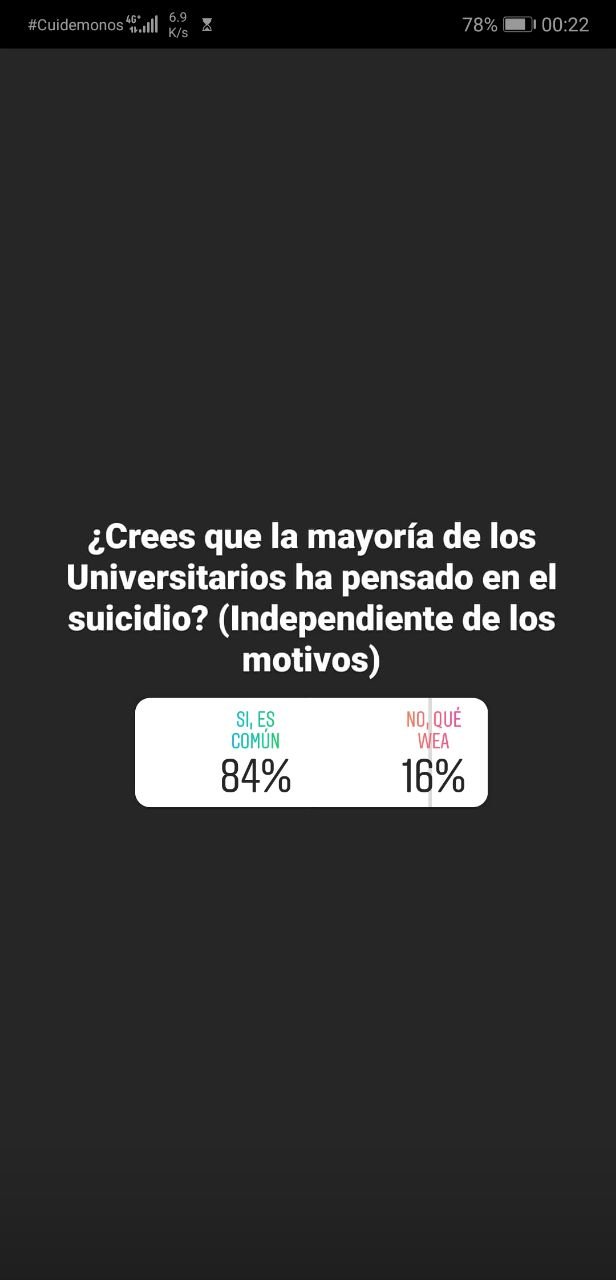
\includegraphics[width=\textwidth]{imgs/insta1.jpg}
    \end{minipage}
    \begin{minipage}{.3\textwidth}
        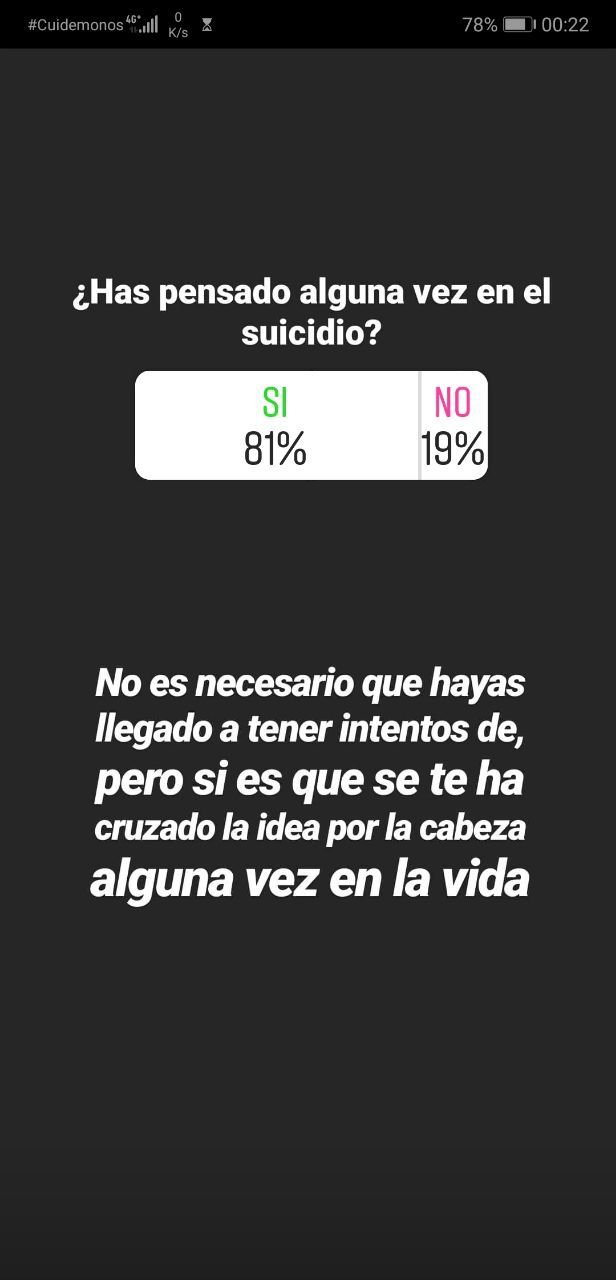
\includegraphics[width=\textwidth]{imgs/insta2.jpg}
    \end{minipage}
    \begin{minipage}{.3\textwidth}
        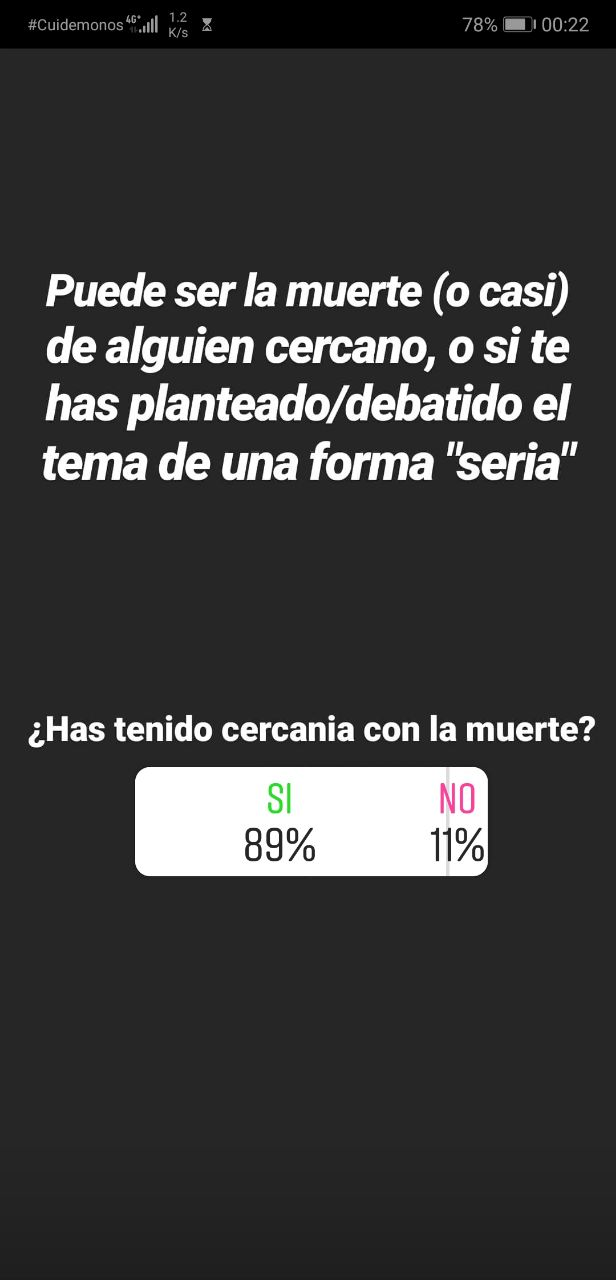
\includegraphics[width=\textwidth]{imgs/insta3.jpg}
    \end{minipage}
    \caption{Encuesta realizada en Instagram}
    \label{fig:instagram}
\end{figure}

La Figura~\ref{fig:instagram} muestra las encuesta realizada a 62 personas, donde la gran mayoría ha tenido cercanía con el suicidio o con la muerte en general. Esto me da la certeza de que no es un dilema que la gente se tome a la ligera y es una temática con la cuál la gente puede empatizar y sentirse identificada.

Trate de buscar investigaciones al respecto (buscando ``videogames and suicide'' y ``suicide in videogames'' para ser precisos) pero solo encontré artículos que hablaban de depresión o riesgos de suicidios asociado a los videojuegos\cite{suicide-risk}, artículos que traían como consecuencia el suicidio pero donde el mismo no era la temática central del juego.

En cambio, en donde si se ha tocado el suicidio, la depresión, y la salud mental en general es en los videojuegos independientes. Buscar ``depression in videogames'' en Google me llevó a un artículo del New York Times\cite{new-york-times} donde muestran como distintos juegos abarcan dificultades mentales desde diferentes ámbitos. Entre ellos cabe mencionar los siguientes:

\begin{itemize}
    \item \textbf{Sea of Solitude} (2019): Un juego donde navegas en una ciudad inundada y donde te enfrentas a la soledad, la desesperanza, la depresión, así como también la protagonista debe enfrentarse a sus propios demonios personales.
    \item \textbf{Celeste} (2018): Un juego de plataformas donde se explora la depresión y la ansiedad a través de la protagonista, quien debe evitar los obstaculos fisicos y emocionales. Sufriendo ataques de ansiedad y siendo perseguida por sus inseguridades.
    \item \textbf{Night in the Woods} (2017): El protagonista vuelve a su pueblo natal después de abandonar la universidad, sin embargo le cuesta volver a interactuar con gente y con viejos amigos, su estado mental se comienza deteriorar y se muestran episodios de un Trastorno de despersonalización.
    \item \textbf{Hellblade: Senua's Sacrifice} (2017): Ambientado en el Siglo VIII, muestra como la protagonista sufre de psicosis -lo que ella cree que es una maldición- y lo que es vivir y lidear con ella.
\end{itemize}

Con toda esta información, se decide elegir el suicidio y la depresión como las temáticas centrales a tratar en el videojuego, y se comienza a trabajar en el diseño y la implementación del mismo, los cuales serán detallados en la Sección~\ref{sec:diseño}.

\begin{figure}
    \centering
    \begin{minipage}{.49\textwidth}
        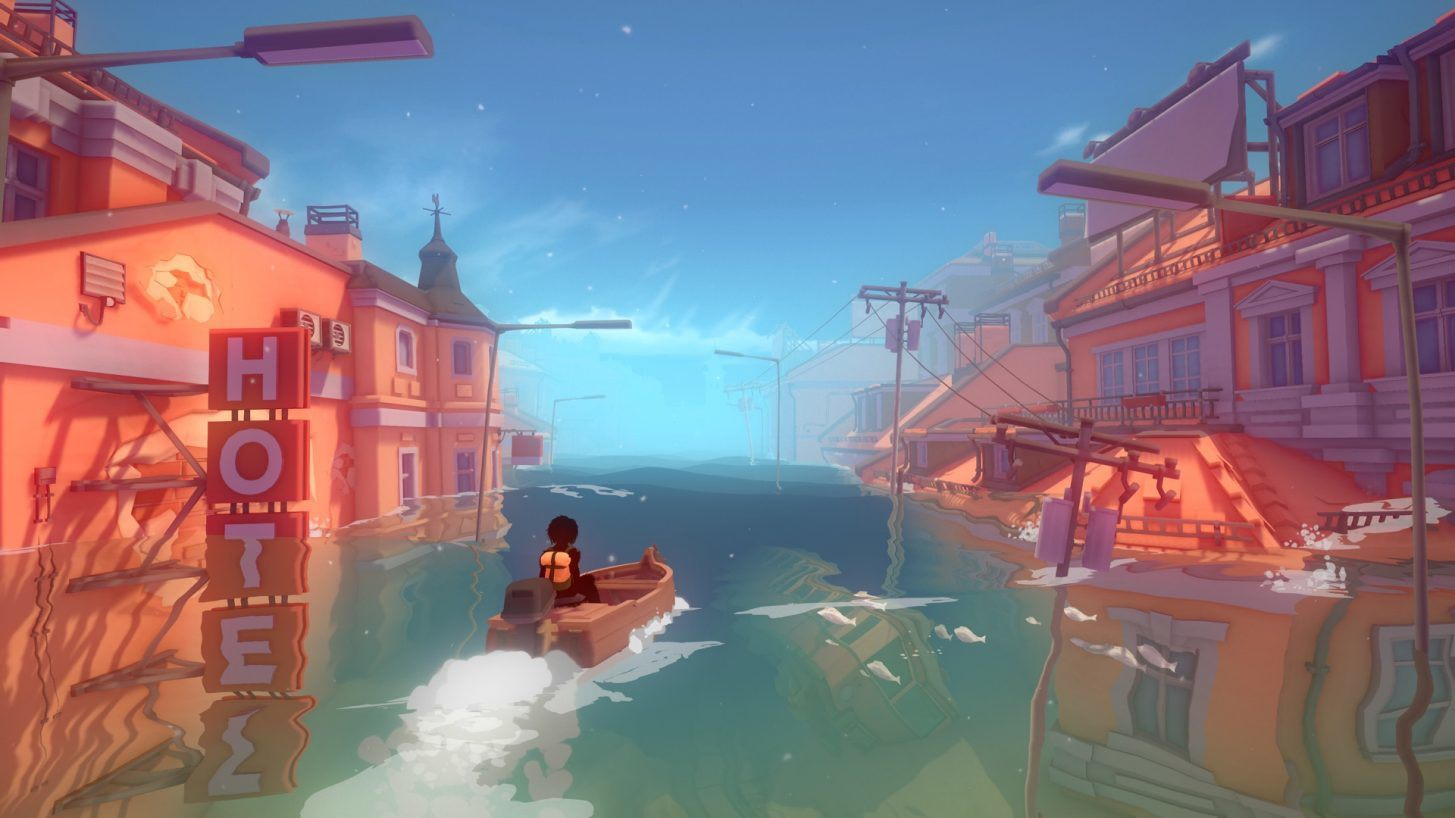
\includegraphics[width=\textwidth]{imgs/sea-of-solitude.png}
        \caption{Sea of Solitude}
        \label{fig:sea-solitude}
    \end{minipage}
    \begin{minipage}{.49\textwidth}
        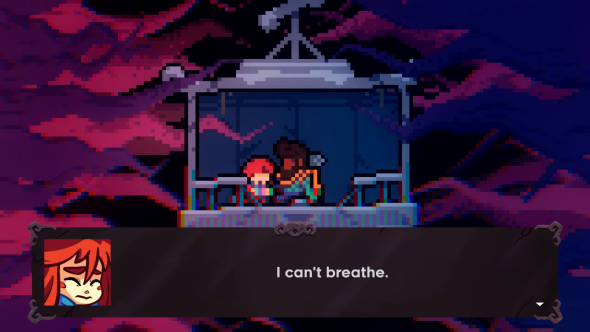
\includegraphics[width=\textwidth]{imgs/celeste_panic_attack.png}
        \caption{Celeste}
        \label{fig:celeste}
    \end{minipage}
\end{figure}
\begin{figure}
    \centering
    \begin{minipage}{.49\textwidth}
        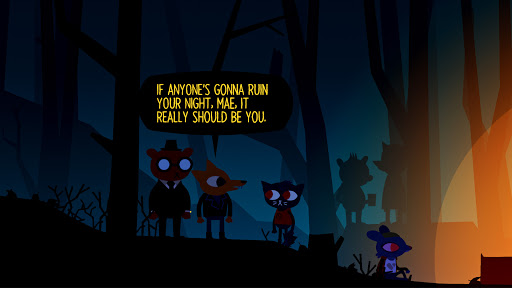
\includegraphics[width=\textwidth]{imgs/night-in-the-woods.jpg}
        \caption{Night in the Woods}
        \label{fig:night-woods}
    \end{minipage}
    \begin{minipage}{.49\textwidth}
        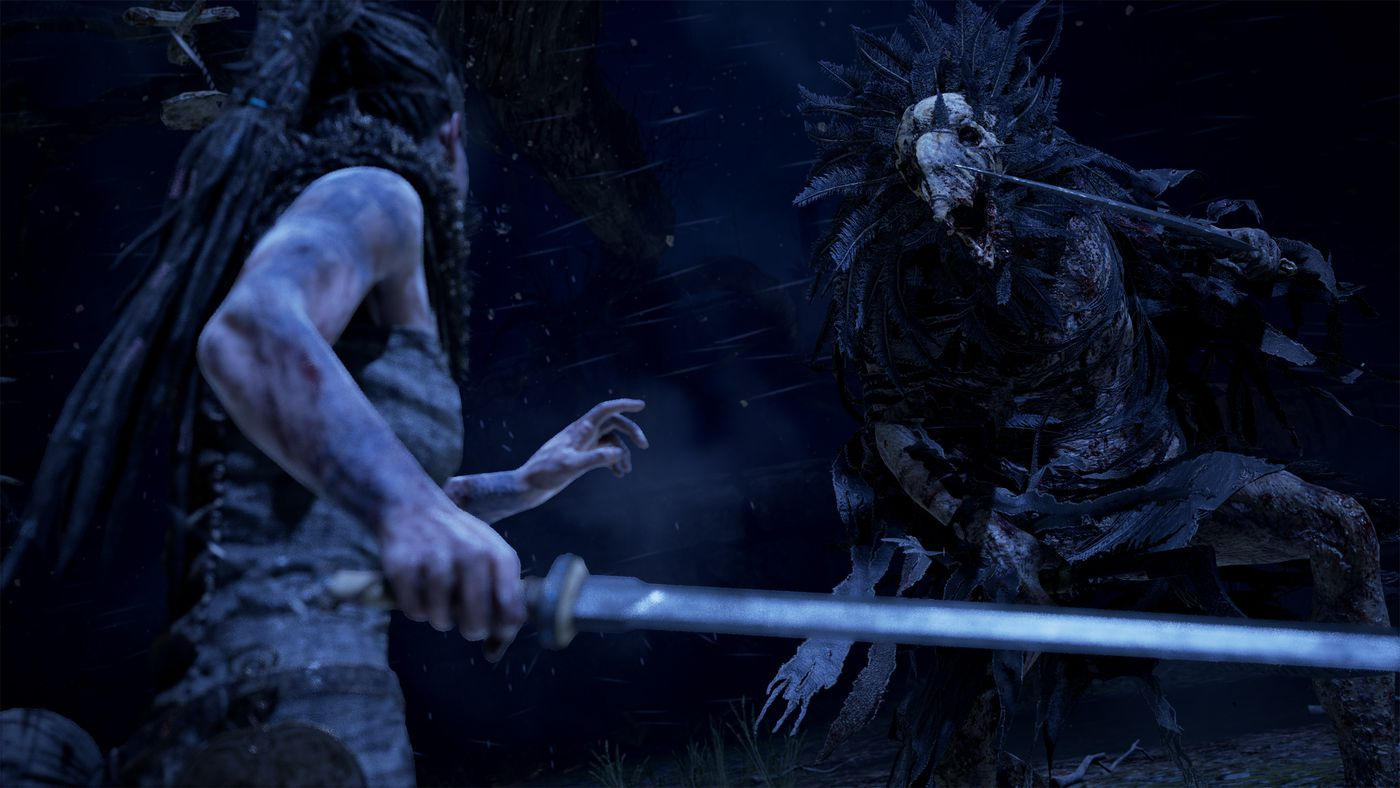
\includegraphics[width=\textwidth]{imgs/hellblade.jpg}
        \caption{Hellblade}
        \label{fig:hellblade}
    \end{minipage}
\end{figure}


%\textbf{Creo que aquí puedes tener en cuenta la búsqueda que has realizado del estado del arte y explicar alguna cosa relacionada con los artículos encontrados y que es lo que quieres hacer tu.
%Creo que también es importante justificar porque te ha interesado el suicidio y ver si se ha hecho algo relacionado. Cuando lo busques recuerda indicar palabras clave de la búsqueda y resultados encontrados}
% Situar al lector en la temática del trabajo

\subsection{Equipo de Trabajo}\label{sec:equipo}
A continuación se detalla el equipo de trabajo que participó en la realización de este proyecto.

\begin{table}[h]
    \centering
    \begin{tabular}{|p{3.5cm}|p{11.5cm}|}
        \hline
        \rowcolor{Gray}
        \multicolumn{2}{|c|}{\textbf{Miembros del Equipo}} \\
        \hline
        \rowcolor{Gray}
        \textbf{Nombre} & \textbf{Rol en el Proyecto} \\
        \hline
        José Francisco Riffo \textit{Tesista} & Desarrollador Principal. Encargado del diseño e implementación del juego así como también de assets graficos secundarios. (UI + Sprites)\\
        \hline
        Karina Olguin & Ilustradora. Encargada de los retratos de cada personaje y de los recuerdos en el minijuego de los puzzles. \\
        \hline
        Imma Boada & Consultora. Se discutieron los detalles del juego y su implementación. \\
        \hline
        Pablo Rojas & Consultor. Se discutieron detalles del tema de la memoria e investigación. \\
        \hline
    \end{tabular}
    \caption{Miembros del Equipo}
    \label{tab:equipo}
\end{table}